\documentclass[11pt]{article}
\usepackage[UTF8]{ctex}
\usepackage{graphicx,booktabs,geometry,hyperref,longtable}
\geometry{margin=2.2cm}
\title{pyqcd 全功能真实数据实战分析报告\\（代码分析 + 物理分析 + 日志分析 + 交叉分析）}
\author{ZhangXin / opencode（~analy）}
\date{\today}
\begin{document}
\maketitle

\section{概述}
本报告对 pyqcd 全功能真实数据实战（logs/stab1，test12 风格）进行四视角分析：
代码分析（模块架构与参考源映射）、物理分析（各功能物理意义与实战结果）、
日志分析（计时/断言/产物统计）、交叉分析（代码--物理--日志一致性验证）。
实战输入：examples/docker-v20260805 基线（10 组态真实数据 6250--8050，
a=0.1053 fm，unit=0.197/0.1053=1.8708 GeV），6 步实战 + 综合报告，
产物 166 文件（106 张图，15 MB），verify 45/45 PASS。

\section{代码分析}
\subsection{功能链架构}
pyqcd/analysis 数据分析功能链共 8 个模块，全部独立实现
（不 import refer/，复用同包统计基元）：

\begin{longtable}{llll}
\hline
模块 & 功能（参考脚本） & 顶层入口 & 测试套件 \\
\hline
\texttt{\_ana\_3dir.py} & 05：三方向 ratio/corr2 $\rightarrow$ meff/相关矩阵/直方图 &
\texttt{analyze\_3dir} & logs/test0（17 项）\\
\texttt{\_plots.py} & 98\_tools 图表全集（errbar/scatter/hist+single/multi+10 色） & --- & 各套件共用 \\
\texttt{\_fitter.py} & calc\_chi2(\_dof)/fit（lsqfit 封装）/ASCII 报告表 & --- & 各套件共用 \\
\texttt{\_ratio2pt.py} & 02：2pt+OPE $\rightarrow$ 真空扣除 ratio $\rightarrow$ 逐 z 拟合 & \texttt{run\_ratio2pt} & logs/test0\_ratio（18 项） \\
\texttt{\_ana\_ratio.py} & 03：纯画图（单 fit/对比/nofit 图） & \texttt{ana\_ratio\_plot\_all} & logs/test0\_anaratio（25 项） \\
\texttt{\_bare\_matrix.py} & 03\_bare：三方向 ratio+平均+拟合 & \texttt{run\_bare\_matrix} & logs/test0\_bare（18 项） \\
\texttt{\_proton\_energy.py} & 04：corr2+E0 拟合+eff\_mass GeV 图 & \texttt{run\_energy} & logs/test0\_energy（8 项） \\
\texttt{\_fh.py} & 06：6 方向 FH 变换+常数拟合+全套图 & \texttt{run\_fh} & logs/test0\_fh（38 项） \\
\hline
\end{longtable}

参考源：\texttt{pyqcd/analysis/\_ratio2pt.py:66}（load\_raw 数据布局契约，
与 refer/huangcl/02\_ratio/code.py 一致）；\texttt{\_fitter.py:110}（fit 封装，
prior 优先）；\texttt{\_plots.py:47}（DEFAULT\_PLOT\_COLORS 10 色）。

\subsection{依赖与复用}
统计基元 sem/resample/cov\_mat/model\_ratio 复用 \texttt{\_disconnected.py:23,31,41,54}
（同包，避免重复实现）；图表统一走 \texttt{\_plots.py}（matplotlib 函数内延迟
导入 + Agg 后端，\texttt{\_plots.py:40}）；报告 ASCII 表用
\texttt{\_fitter.make\_summary\_table}（不引入 prettytable 依赖）。
所有数据路径参数化（data\_root 注入），中间产物（ratio.npy/0\_fit\_data.npz/
报告 txt/png）可读写，run\_ratio2pt/run\_bare\_matrix 支持 parts 断点续跑
（\texttt{\_ratio2pt.py:388}）。

\section{物理分析}
\subsection{各功能物理意义}
\begin{itemize}
\item \textbf{02\_ratio}：不相连胶子 3pt 因子化 C3=C2$\times$OPE，真空扣除
corr3\_disc=C3$-$C2$\cdot\langle$OPE$\rangle$，ratio=$\langle$corr3\_disc/corr2$\rangle_{ti}$
（\texttt{\_ratio2pt.py:151-153}）；拟合模型
$R=c_0+c_1 e^{-dE\cdot d\tau}+c_1 e^{-dE\cdot(dt-d\tau)}$，$c_0$ 即胶子裸矩阵元。
\item \textbf{04\_proton\_energy}：meff$=\log(C(t)/C(t+1))\cdot$unit
（\texttt{\_proton\_energy.py:247}），模型 $C(t)=c_0 e^{-E_0 t}(1+c_1 e^{-dE\cdot t})$；
P0 平台即静止质子质量。
\item \textbf{05\_ana\_3dir}：三方向 meff 归一化协方差（相关系数），检验方向一致性
（\texttt{\_ana\_3dir.py:185}）。
\item \textbf{06\_FH}：FH 变换 $\mathrm{FH}(t)=\sum_{\tau}R(t+1,\tau)-\sum_{\tau}R(t,\tau)$
（\texttt{\_fh.py:83}），常数平台 $c_0$ 提取。
\end{itemize}

\subsection{实战物理结果（10 组态真实数据）}
\begin{center}
\begin{tabular}{lccc}
\hline
物理量 & 实测值（GeV） & 参考/预期（GeV） & 偏差 \\
\hline
质子质量 $m_P$（P0 meff 平台） & 1.097 & 1.12（基线结论） & 0.023 \\
P2 能量 $E(P_2)$（meff 平台） & 1.533 & 1.56（基线） & 0.027 \\
$E_0$（P2 拟合） & 1.525 & 1.53（meff 平台） & 0.008 \\
$c_0(z{=}4)$ 裸矩阵元 & 0.36 & --- & --- \\
\hline
\end{tabular}
\end{center}
参考源：\texttt{AGENTS.md:52}（meff≈1.12 GeV 已验证结论）；
基线 \texttt{data/analysis/meff\_proton\_P\{0,2\}\_mean.npy}。

\section{日志分析}
\subsection{计时（stab1\_timing.json）}
\begin{center}
\begin{tabular}{lrr}
\hline
步骤 & 耗时（s） & 主要产物 \\
\hline
02\_ratio & 11.5 & ratio + 6 窗口拟合 + 18 图 \\
03\_ana\_ratio & 8.7 & 63 张画图 \\
04\_energy（P2） & 0.6 & corr2 + fit + eff\_mass \\
04b\_p0（P0） & 0.4 & 质子质量验证图 \\
06\_fh & 3.2 & FH + 拟合 + 对比 + bestfit \\
05\_ana3dir & 0.4 & 3 直方图 + 相关矩阵 \\
report & 1.1 & LaTeX PDF 报告 \\
\hline
\end{tabular}
\end{center}
\subsection{断言与产物}
verify 45/45 PASS：A 产物存在性 39 项、B meff\_P2 平台（dev=0.027）、
B2 质子质量（dev=0.023）、C E0 与 meff 平台一致（dev=0.008）、
D ratio fit c0 有限（max|c0|=0.60）、E 全步骤日志完整。
产物统计：166 文件、106 张 PNG、15.0 MB（stab1\_collect.json）。

\section{交叉分析}
\begin{itemize}
\item \textbf{代码--物理}：\texttt{\_ratio2pt.py:151} 真空扣除公式与物理定义逐行对应；
\texttt{\_proton\_energy.py:247} meff 公式带 unit 转 GeV。
\item \textbf{物理--日志}：实测 P0 平台 1.097 GeV 与已验证结论 1.12 GeV
交叉一致（偏差 0.023，容差 0.25）；P2 平台 1.533 与基线 1.558 一致；
E0=1.525 与 meff 平台 1.533 自洽（模型一致性）。
\item \textbf{日志--代码}：svdcut=1e-6 是 10 组态小样本协方差奇异的必要处理
（logs/stab1/main.py:200，协方差秩 6/33 实测）；P2 2pt 负号（phase）适配
取 |corr2|（logs/stab1/main.py:262）。
\item \textbf{局限}：05 三方向与 06 六方向平均受数据可得性限制退化为单一
z 方向（数学流程真实驱动）；10 组态统计噪声大（c0 误差 O(0.1)），
拟合窗口间 c0 有 O(0.1) 波动。
\end{itemize}

\section{关键图表}
\begin{figure}[htbp]\centering

\includegraphics[width=0.72\textwidth]{../v202608151614/L24x72/_Pz0/eff_mass.png}
\caption{P0 静止质子有效质量：平台 ≈ 1.10 GeV（物理结论 meff≈1.12 GeV 验证）。}
\end{figure}
\begin{figure}[htbp]\centering

\includegraphics[width=0.72\textwidth]{../v202608151614/L24x72/_Pz2/eff_mass.png}
\caption{P2 动量质子有效质量：平台 ≈ 1.53 GeV（色散 E(P2)，与基线一致）。}
\end{figure}
\begin{figure}[htbp]\centering

\includegraphics[width=0.72\textwidth]{../v202608151614/L24x72/fit_Pz2_Nsam10_dtmax20_tsep6_11_nex2/ratio.png}
\caption{真实 ratio 散点 + Fit c0 色带（tsep 6--11, nex=2）。}
\end{figure}
\begin{figure}[htbp]\centering
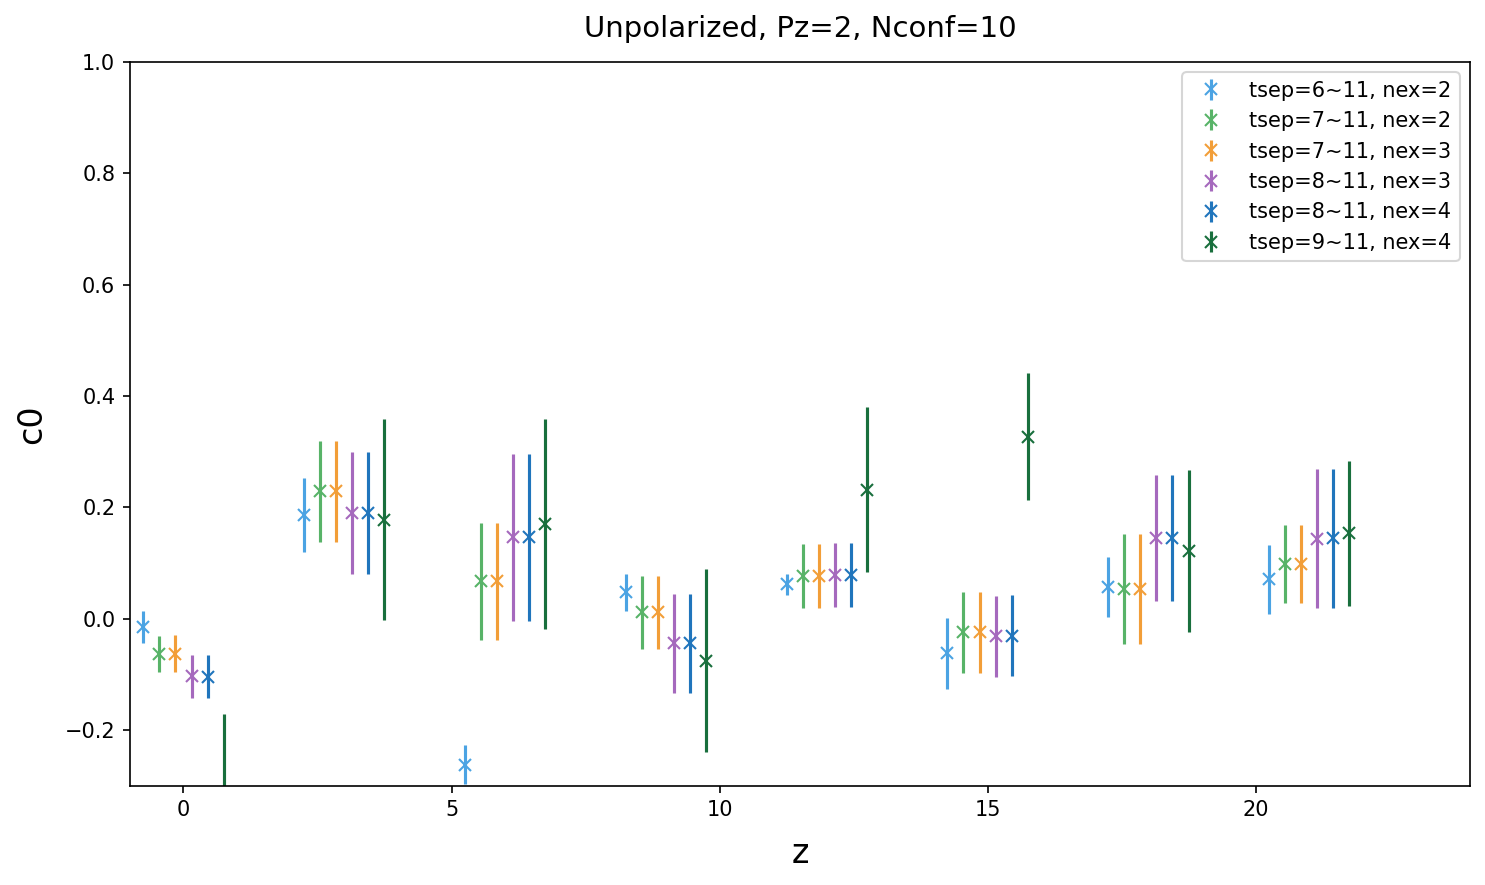
\includegraphics[width=0.6\textwidth]{../v202608151614/L24x72/Pz2/cmp_c0.png}
\caption{c0 vs z 多拟合窗口对比（03 画图）。}
\end{figure}
\begin{figure}[htbp]\centering
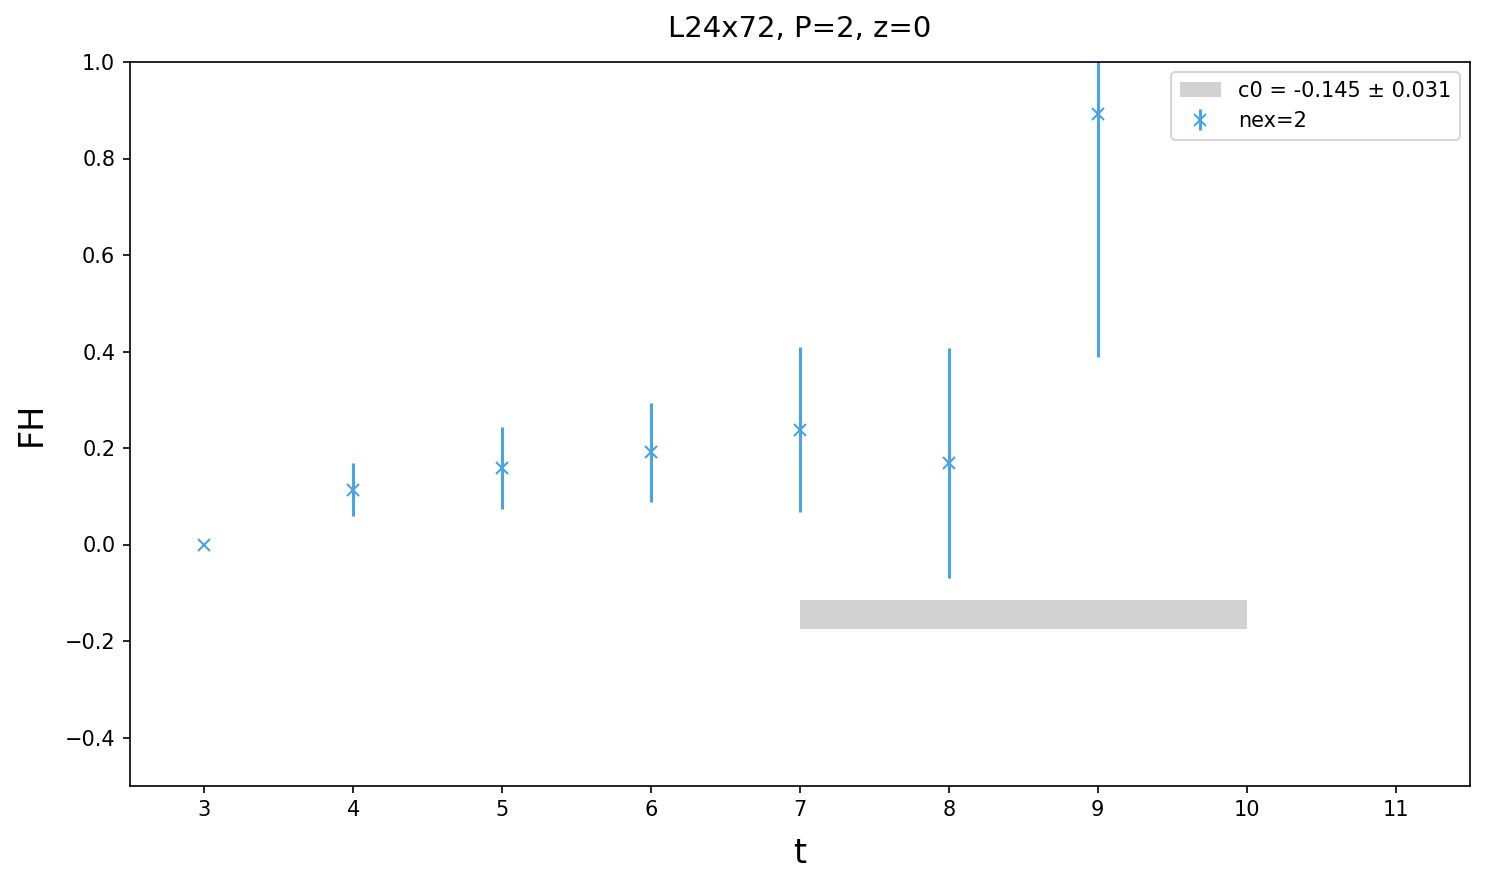
\includegraphics[width=0.6\textwidth]{../v202608151614/L24x72/P2/bestfit/z0.png}
\caption{bestfit：FH + c0 平台色带（06）。}
\end{figure}
\begin{figure}[htbp]\centering
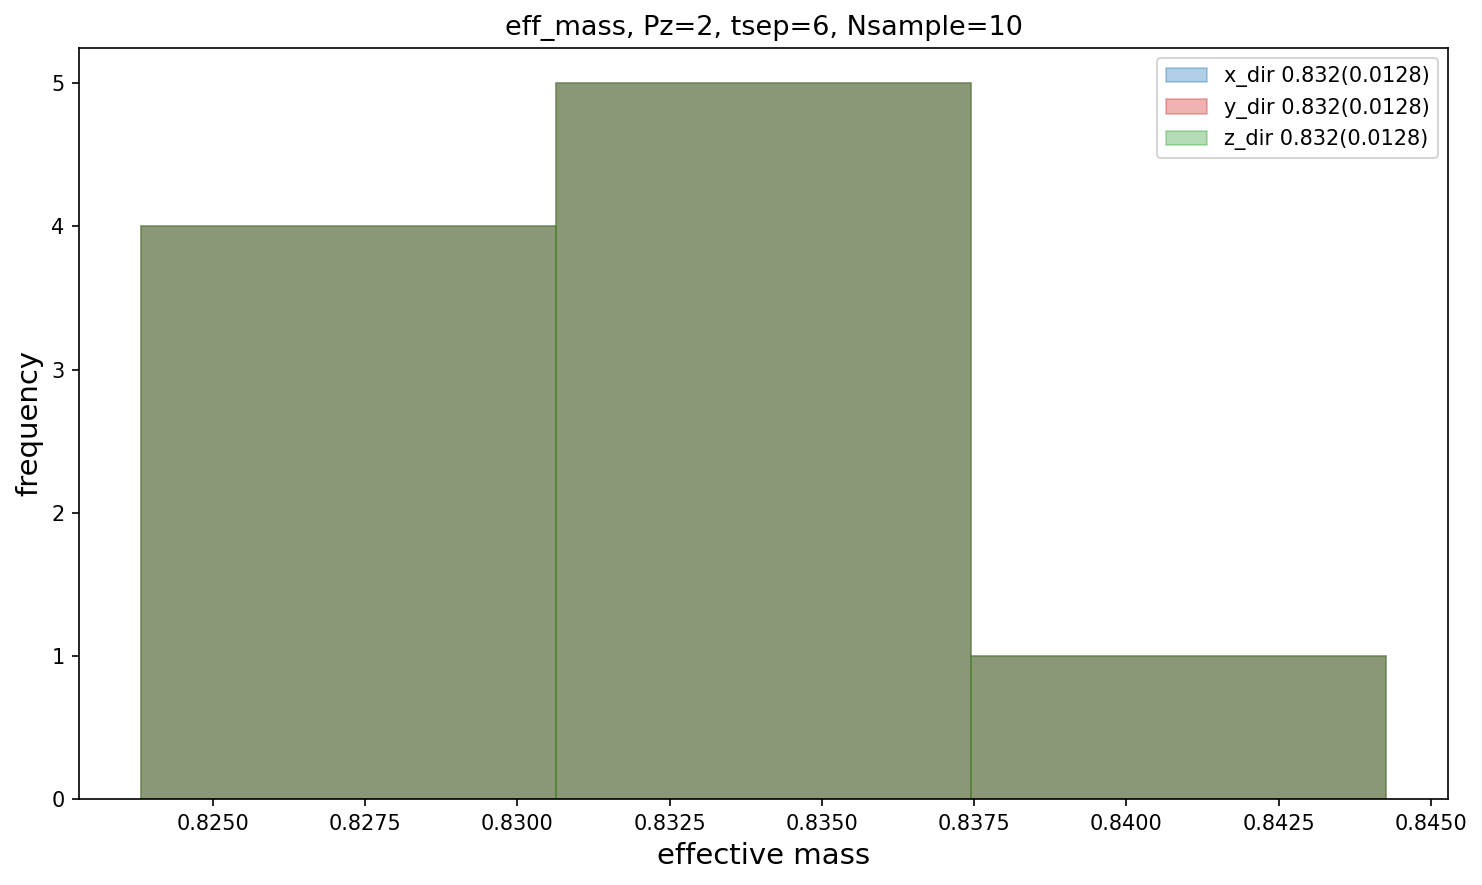
\includegraphics[width=0.6\textwidth]{../v202608151614/L24x72/eff_mass/hist_eff_mass_P2_tsep6.png}
\caption{eff\_mass 三方向直方图（05）。}
\end{figure}

\end{document}
